\documentclass[12pt]{article}

\usepackage{times}
\usepackage{ifpdf}
\ifpdf
\usepackage[pdftex]{graphicx}
\else
\usepackage{graphicx}
\fi

\usepackage{minitoc}
\usepackage{subfigure}
\usepackage{color}
\usepackage{url}
\usepackage{latexsym}
\usepackage{geometry}
\usepackage{indentfirst}
\usepackage{array}
\usepackage{tabularx}
\usepackage{xtab}
\usepackage{fancyvrb}
\usepackage[center, bf]{caption}
\usepackage{listings}
\usepackage{url}
\usepackage{placeins}

\begin{document}
\begin{titlepage}
	\centering
	\begin{figure}[ht]
		\centering
		% TODO fix latex errors
		
\includegraphics[angle=-90, keepaspectratio=true, width=8cm]{logo}
	\end{figure}
	{
	\large \bfseries Nomadic Comunication\par
	AA 2008-2009
	}\par
	\vspace{1.5cm}
	{
	\Large \bfseries \textcolor{blue}{Report 1: The tile!} \par
	}
	\vspace{1.0cm}
	{
	\large \bfseries {Group N. XXX} \par
	}
	\vspace{0.3cm}
	{
	\large \bfseries {Author 1, author 2, etc...}
	}
	\vspace{1.0cm}
	\begin{abstract}
	%Abstract here.
	\end{abstract}
\end{titlepage}

\thispagestyle{empty}
\tableofcontents
\clearpage
\setcounter{page}{1}

%%%%
% Usefull things in latex:
% itemize, enumerate, lstlistings (to report source code, shell output, whatever), emph, tables
%
%%%
% How to include a single figure:
%	\begin{figure}
%		\begin{center}
%			\includegraphics[width=1\textwidth]{path/to/image_file} % use "image_file" for "image_file.pdf"
%			\caption{Tor average transfer time comparison between different CW sizes on server side.} \label{fig:speed}
%		\end{center}
%	\end{figure}
%
%%%
% TODO
% - Refer to Professor template for some usefull hints: http://disi.unitn.it/locigno/index.php/teaching-duties/nomadic-communications/aa08-09
% - *Always* use \cite and \ref when needed. Adding it when the text is already written is senseless waste of time, the result will be hugly.
% - Use \footnote if necessary, it can make things more readable.
% - Please indent your Latex code! Use tabs, not spaces.
% - English! Write in grammatically correct English. (Aspell can check latex source files)
% - This is a formal document that requires formal writing. This means that "it's", "I've", "ain't" and others must be replaced by their extended form.
% - Use \emph the first time you call something new or when you introduce a new abbreviation i.e.: Internet Protocol (\emph{IP}). Do not abbreviate access point to AP in descriptions and similar
%
%%%%
% IMPORTANT
% Every section is writte in a separate file (see \include commands). This means that anything (subsections and everything else) following \include should be placed in that file. I wrote everything here to make the thing readable.

\section{Introduction} \label{intro}
	% Describe what we are gonna do, the general ideas and what we are gonna talk about.
% Say what is needed to understand the sections that will follow.

The purpose of the project 
is the evaluation of the performances variation of a wireless network 802.11 b/g at the change of some parameters.
\\\newline
In order to make those tests we used some tools whitch are Iperf, wireshark, and a complex python script for the automated run test.
\\\newline
The test consist basicaly in many automatic execution of iperf with fixed time and different speed and finaly we consider the amount of transfering data.
\\\newline
The set of the tests was an indoor environment a notebook wich run iperf as server, an other notebook wich run iperf as client (throw the python script), a cisco ap and another notebook wich run wireshark to sniff the traffic.

\vspace{1cm}

\begin{figure}[h!]
	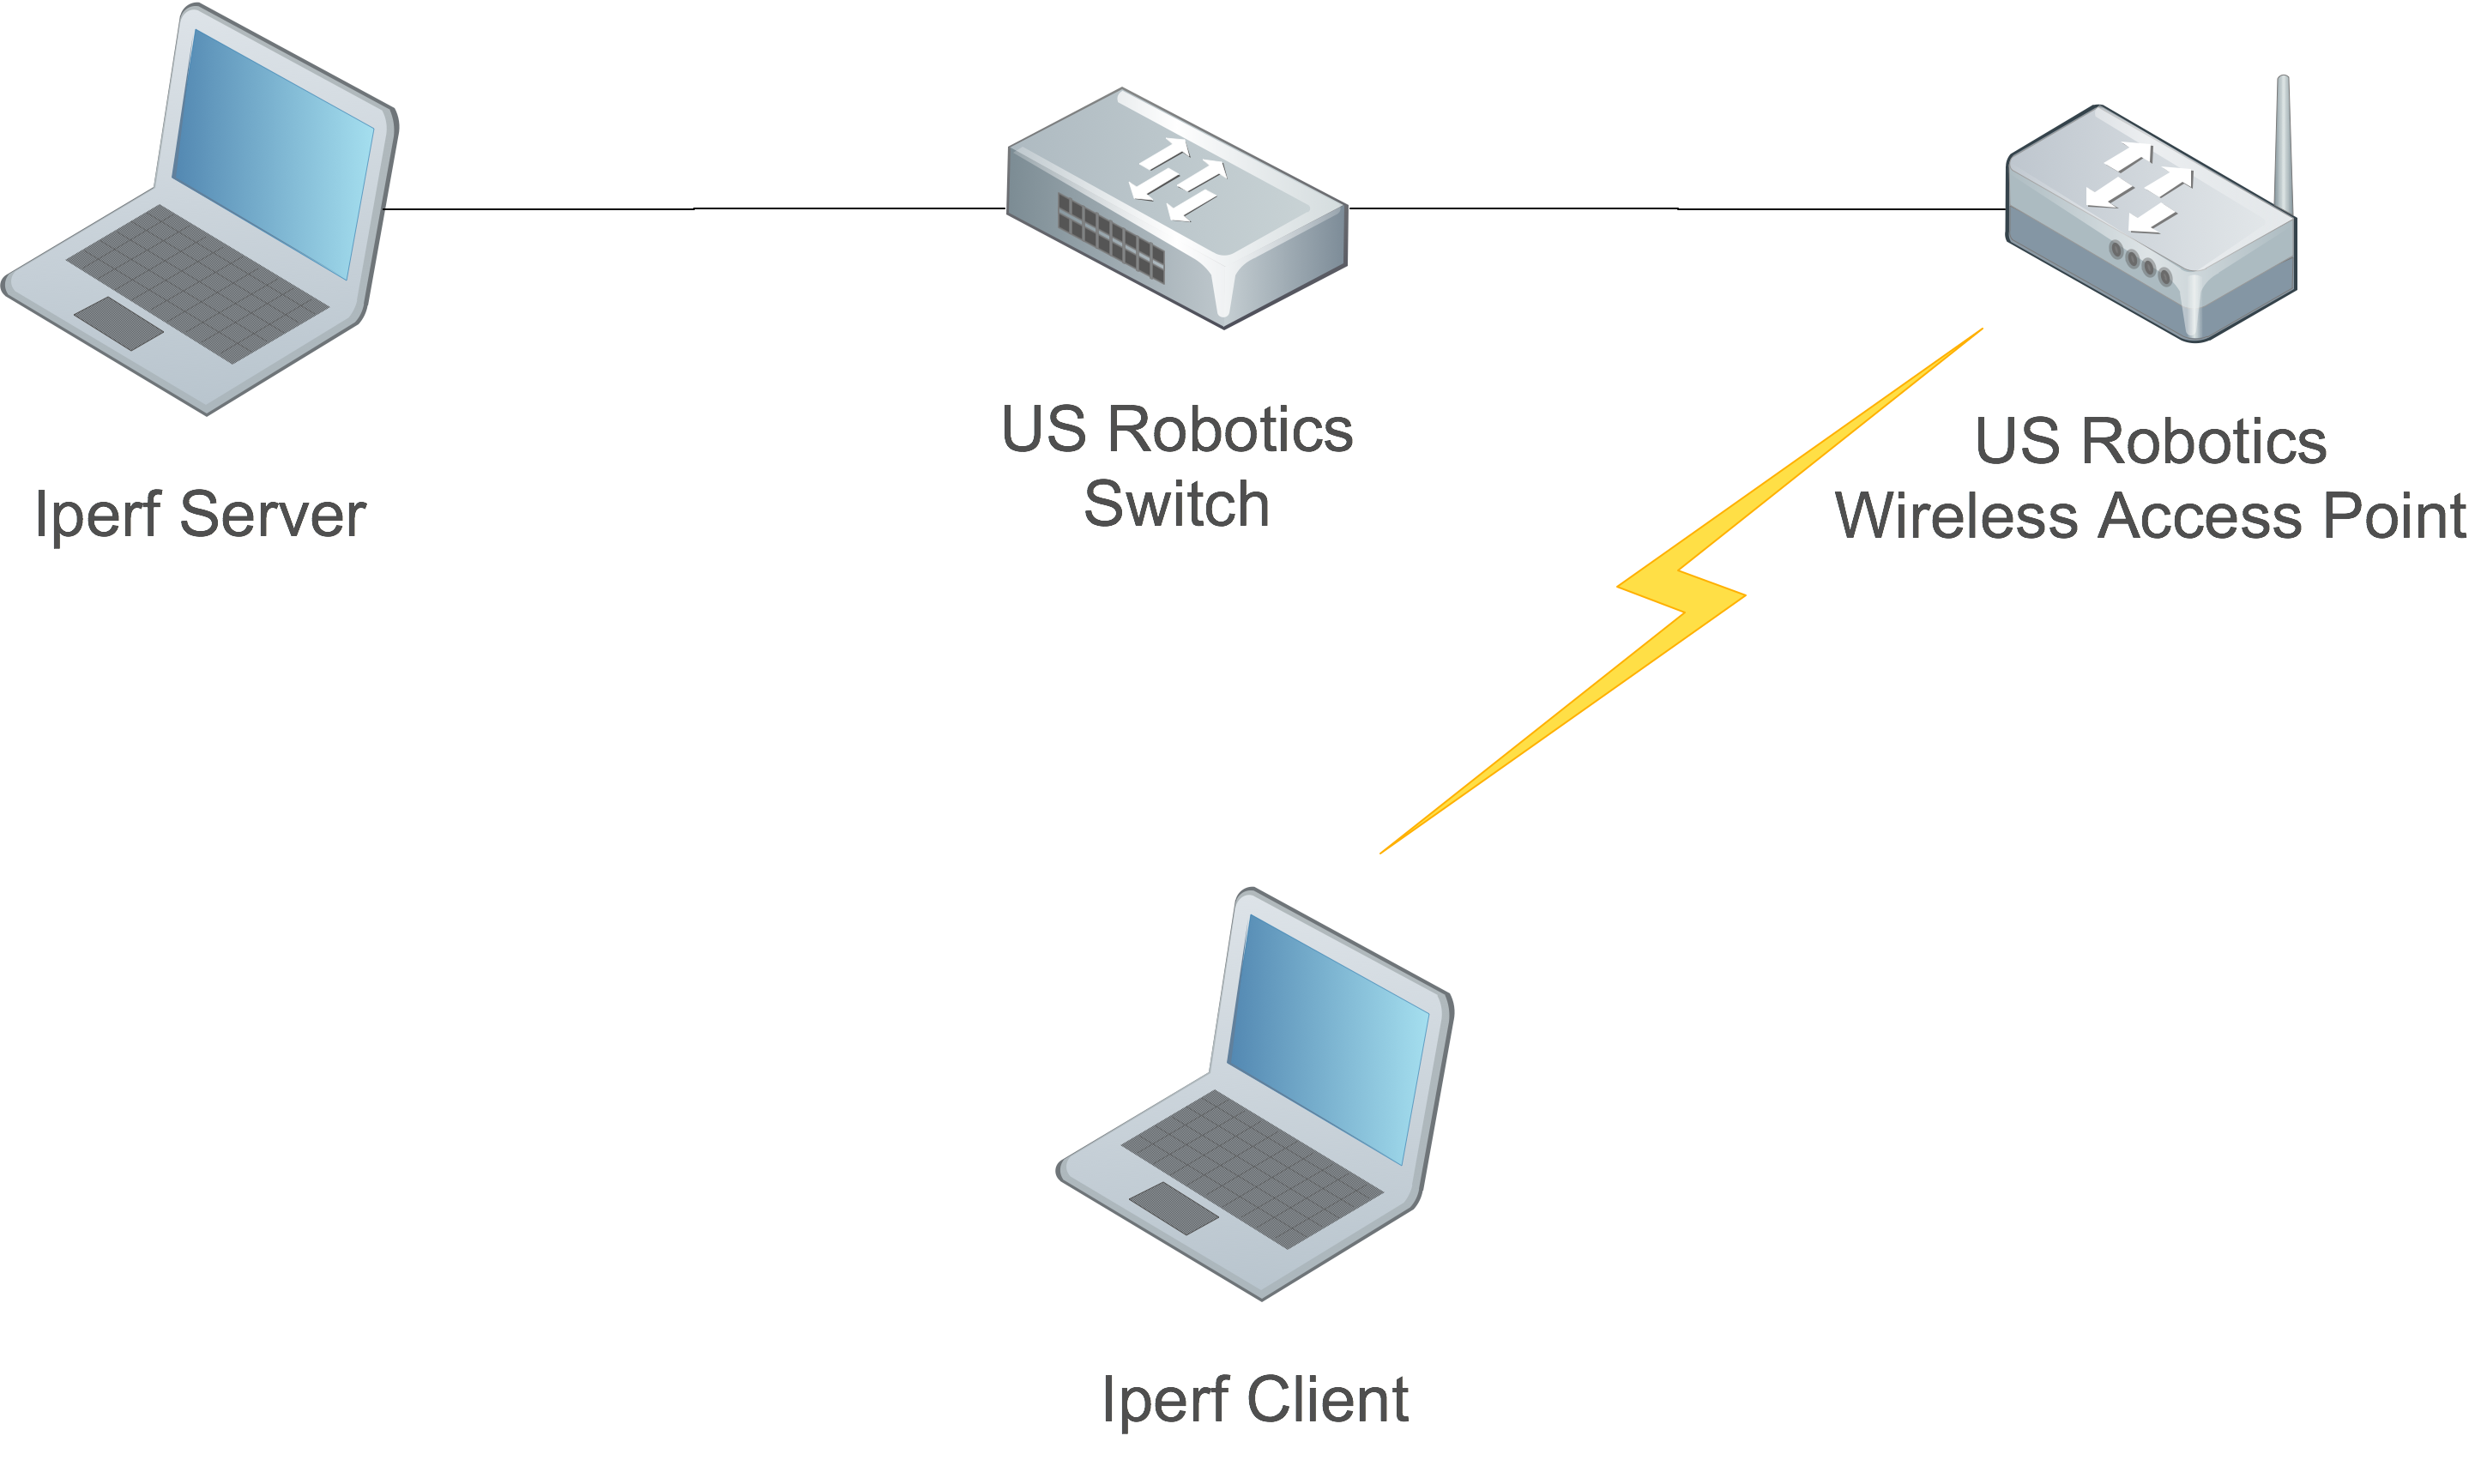
\includegraphics[angle=0, keepaspectratio=true, width=15cm]{images/network_overview}
	\caption{Network overview}
\end{figure}

	% Describe what we are gonna do, the general ideas and what we are gonna talk about.
	% Say what is needed to understand the sections that will follow.

\section{Theoretical background} \label{theory}
	% Everything that comes from theory and that is needed to understand and describe our work.
	\subsection{802.11} \label{theory:prot_specs}
	802.11 is the standard family of protocols for wireless networks. It is also named Wi-Fi. 802.11 protocols family describe how various wireless devices must interact. Nowadays the most popular 802.11 implementation are 802.11b and 802.11g.
	
% A simple description of how an IEEE 802.11 protocol works to introduce the fact that there is some overhead added by the protocol.
% Yes, I know it's unbelivable but there are some differences, for real! :)
	\subsection{Differences between 802.11b and 802.11g} \label{theory:prot_differences}
	
	802.11b protocol was born in October 1999 and since this date it has a discrete success but with the advent of some other wireless device such as cordless telephones it suffer interfernce that causes slower performance. 802.11b extends the basic net bit rate of the standard 802.11 up to 11 Mbit/s.\\
	
	In June 2003 arrives 802.11g that is fully backwards compatible with 802.11b but has best bit rates and throughput\\
	Both protocols use the same frequency band (2.4 GHz) but use different frequency spreads. While 802.11b use direct sequence spread spectrum signaling (DSSS), 802.11g use orthogonal frequency division multiplexing (OFDM) methods. Because of OFDM 802.11g increase the net bit rate up tu 54 Mbit/s.
	
	\begin{table}[h]
		
		\begin{tabularx}{15cm}{ | X X X X X X | }
			\hline
				802.11 Protocol & Release & Freq. (GHz) & Typ throughput (Mbit/s) & Max net bitrate (Mbit/s) & Modulation \\
			\hline
				-- & Jun 1997 & 2.4 & 00.9 & 002 & DSSS \\
				b & Sep 1999 & 2.4 & 04.3 & 011 & DSSS \\
				g & Jun 2003 & 2.4 & 19 & 054 & OFDM \\
			\hline
		\end{tabularx}
		
		\caption{802.11 family standard}
		\label{802.11_family_standard}
	\end{table}
	
	As we can see from the table the standard g's typical throughput is just shy of fivefold then b standard typical throughput and the main difference is the modulation method.

		% Calculate protocols upperbound limitations and similar things (report the formulas!).
		% DO NOT USE PROFESSOR SLIDES AS SOURCE OF INFORMATIONS SINCE MOST OF VALUES ARE COMPLETELY WRONG!!!!!!!!!
		% Download the IEEE standard from here: http://disi.unitn.it/locigno/didattica/NC/802.11-2007.pdf and make a large use of ^F.

	% Everything that comes from theory and that is needed to understand and describe our work.
	% A simple description of how an IEEE 802.11 protocol works to introduce the fact that there is some overhead added by the protocol.
		%\subsection{Differences between 802.11b and 802.11g} \label{theory:prot_differences}
			% Yes, I know it's unbelivable but there are some differences, for real! :)
			% Calculate protocols upperbound limitations and similar things (report the formulas!).
			% DO NOT USE PROFESSOR SLIDES AS SOURCE OF INFORMATIONS SINCE MOST OF VALUES ARE COMPLETELY WRONG!!!!!!!!!
			% Download the IEEE standard from here: http://disi.unitn.it/locigno/didattica/NC/802.11-2007.pdf and make a large use of ^F.

\section{Testbed Setup} \label{setup}
	% Say what is the testbed used for tests including *everything* necessary, both hardware, software, hardware position, air humidity and everything meaningful for the tests.
	%
	% We have used 2 pc (client C and server S), 1 access pocp reint (AP) and 1 switch. The idea is simple:
	% - AP, C and S are connected to the switch on a wired LAN
	% - we use 2 separate class C LANs (wlan and clan):
	%      one for wired traffic like retriving tcpdump and iperf outputs
	%      the other one for the wireless tests
	% - C connects to S via SSH over clan, starts iperf server and starts tcpdump
	% - C uses iperf to send UDP traffic to S over AP on wlan
	% - C gets out outputs from S using clan
	\subsection{Hardware} \label{setup:hardware}
	% mainly C wifi card configuration, ap settings

\noindent
For the experiment we were provided with some devices by the university, however, we decided to use our own equipment for doing the tests.

Our iperf server and client were run on different notebooks, as shown in table \ref{tbl:laptops}. Furthermore, the network consists of an US Robotics Access Point and a switch from the same company (table \ref{tbl:networkdevices}).


%\subsubsection{Laptops}
%	\begin{tabular*}{1\textwidth}{@{\extracolsep{\fill}} | l l | }
	\begin{table}[h]
		
		\begin{tabularx}{15cm}{ | m{4cm} X | }
			\hline
				ROLE & Client\\
				MODEL & HP Pavilion dv5-1070el\\
				WIFI & Intel PRO/Wireless 5100 AGN\\
				FIRMWERE & iwlwifi-5000 - 6 October 2008\\
			\hline
		\end{tabularx}
		\\\\\\
		\begin{tabularx}{15cm}{ | m{4cm} X | }
			\hline
				ROLE & Server\\
				MODEL & Asus M2410L\\
				WIFI & Intel PRO/Wireless LAN 2100 3B Mini PCI\\
				FIRMWERE & ipw2100\\
			\hline
		\end{tabularx}
		
		\caption{Laptop configuration}
		\label{table1}
		\label{tbl:laptops}
	\end{table}

%\subsubsection{Network devices}
	\begin{table}[h]
		
		\begin{tabularx}{15cm}{ | m{4cm} X | }
			\hline
				ROLE & Access Point\\
				MODEL & US Robotics 805450\\
				FIRMWERE & version 1.53\\
			\hline
		\end{tabularx}
		\\\\\\
		\begin{tabularx}{15cm}{ | m{4cm} X | }
			\hline
				ROLE & Switch\\
				MODEL & US Robotics\\
			\hline
		\end{tabularx}
		
		\caption{Network devices configuration}
		\label{table2}
		\label{tbl:networkdevices}
	\end{table}

	%\subsection{Hardware} \label{setup:hardware}
		% mainly C wifi card configuration, ap settings

	\subsection{Software} \label{setup:software}
	% ssh keys, iwconfig, python software, iperf, tcpdump, gnuplot, whatever used

	%\subsection{Software} \label{setup:software}
		% ssh keys, iwconfig, python software, iperf, tcpdump, gnuplot, whatever used

\subsection{Parameters} \label{parameters}
	% Parameters of the tests. Everything that influences the tests and the results we are trying to look at. This includes both static and variables things.
% Wifi channel speed used, fragmentation threshold, rst threshold and similars

	% Parameters of the tests. Everything that influences the tests and the results we are trying to look at. This includes both static and variables things.
	% Wifi channel speed used, fragmentation threshold, rst threshold and similars

\section{Results} \label{results}
	The tests we executed are in order
%(andrea/tests)s

\begin{figure}
    
\end{figure}
	% Our results and something that underlines that we understand the mean of the results. Results are not self evident!
	% Any formula used to calculate the efficency or whatever must be written and described.
	%\subsection{IEEE 802.11b} \label{resutls:11b}
	%\subsection{IEEE 802.11g} \label{resutls:11g}

\section{Conclusion} \label{concluion}
	% Conclusion must say what we understand from our results, what is the learned lesson and so on.

\addcontentsline{toc}{section}{Bibliography}
\bibliographystyle{plain}
\bibliography{biblio} % put bibliografy in a file called biblio.bib
% Include all books, manuals, softwares home pages etc used for the tests.
% Including links to wikipedia is like saying that we are a bunch of fools... better not to :)
\nocite{*}
\appendix % if necessary
% We should do something for Andrea's software...
\end{document}
